\documentclass{article}
\usepackage{graphicx} % Required for inserting images
\usepackage[T1]{fontenc}
\usepackage[polish]{babel}
\usepackage[utf8]{inputenc}
\usepackage[a4paper, total={6in, 8in}]{geometry}
\usepackage{markdown}
\usepackage{float}
\graphicspath{{images/}}

\title{Dokumentacja PWI}

\author{Kyrylo Goroshenko \and 
Olaf Surgut\\
\and 
Szymon Kuczyński\\
(Kucz) 
\and
Lidia Podoluk
\and
Piotr Wasielewski
\and
Łukasz Janicki\\
\and
Aliaksandr Luksha
}

\begin{document}

\maketitle
\section{Czego dotyczy projekt}

W projekcie stworzona została aplikacja do gry w pokera tajskiego. Główna część dokumentacji dotyczy technicznych aspektów aplikacji i jej obsługi. Zasady gry są opisane na końcu jako część dodatkowa.\\
Aplikacja składa się z dwóch elementów: serwera oraz klienta.

\section{Uruchamianie aplikacji}
\subsection{Uruchamianie serwera}
Należy zainstalować wymagane pakiety wykonując w terminalu komendy:\\
\texttt{sudo apt install python3}\\
\texttt{pip install -r requirements.txt}\\
Następnie należy zmienić domyślne ustawienia serwera.\\
W pliku \texttt{config.py} należy zmienić wartość pola \texttt{"host"} na IP serwera (być może lokalne) oraz \texttt{"port"} na dowolny wybrany (domyślnie 5000).\\
Serwer uruchamia się za pomocą komendy\\
\texttt{python3 server.py}\\

\subsection{Uruchamianie gry}
Aby uruchomić grę, należy znajdować się w folderze głównym repozytorium oraz wykonać w terminalu komendę:\\
\texttt{python3 main.py}\\
Gra sama uruchomi klienta i połączy się z serwerem, ale \textbf{należy się upewnić, że jakiś serwer jest już postawiony}, bo inaczej klient wyłączy się i gra się nie uruchomi.

\section{Dokumentacja techniczna}

\subsection{Folder \texttt{logic}}
Folder \texttt{logic} zawiera kody opisujące zasadniczą logiczną część gry.

\subsubsection{\texttt{cards.py}}
Plik \texttt{cards.py} zawiera słowniki opisujące kolory i figury kart oraz prostą klasę \texttt{Card} wykorzystywaną w innych kodach.

\subsubsection{\texttt{player.py}}
Plik \texttt{player.py} implementuje klasę \texttt{Player}, która posiada szereg atrybutów wykorzystywanych przez serwer oraz klienta i potrzebnych do kontrolowania przebiegu gry.

\subsubsection{\texttt{deck\_of\_cards.py}}
Plik \texttt{deck\_of\_cards.py} implementuje klasę \texttt{Deck}, wykorzystywaną do losowania rozdań i kontrolowania ich przebiegu poprzez pamiętanie rozdanych kart.

\subsubsection{\texttt{setcheck.py}}
Plik \texttt{setcheck.py} zawiera zestaw funkcji sprawdzających, czy dany układ znajduje się w danym zbiorze kart. W praktyce tym zbiorem zawsze są karty rozdane graczom w turze, przechowywane w zbiorze \texttt{dealt} będącym atrybutem klasy \texttt{Deck}.

\subsubsection{\texttt{bids.py}}
Plik \texttt{bids.py} zawiera słownik możliwych odzywek licytacyjnych w postaci stringów, którym odpowiadają inne stringi będące wywołaniami funkcji z \texttt{setcheck.py}.

\subsubsection{\texttt{game\_start.py} i \texttt{table.py}}
Pliki te implementują klasę \texttt{Table}, która przechowuje informacje na temat graczy, odzywek (\textit{bidów}) i talii kart. Posiada również funkcje takie jak rozpoczęcie gry (wykorzystuje do tego kod z \texttt{game\_start.py}) lub jej zakończenie, dodanie lub usunięcie gracza, przygotowanie i rozpoczęcie następnej tury, funkcję zwracającą identyfikator obecnego gracza (na potrzeby komunikacji klient-serwer). Oprócz tego klasa \texttt{Table} posiada także funkcję do składania  bidów, która zawiera kod z \texttt{check.py}, oraz funkcje wyświetlające historię odzywek i odzywki dostępne dla gracza.

\subsection{Foldery \texttt{client}, \texttt{server} oraz plik \texttt{config.py}}

\subsubsection{\texttt{config.py}}
W pliku tym znajdują się jedynie informacje na temat IP hosta oraz portu. Wartości te należy zmienić odpowiednio dla użytkownika, w zależności od tego, gdzie chce się postawić serwer.

\subsubsection{\texttt{client}}
Jedynym elementem zawartości tego folderu jest plik \texttt{client.py}. Zawiera on szereg funkcji, które komunikują się z serwerem i zwracają potrzebne informacje z odpowiedzi serwera. Plik ten posiada także prosty interfejs terminalowy służący do testowania komunikacji klient-serwer.

\subsubsection{\texttt{server}}
Jedynym elementem zawartości folderu \texttt{server} jest plik \texttt{server.py}, który korzysta z Flaska, aby utworzyć serwer do gry. Serwer ten posiada bazę danych graczy i stołów (odpowiednio \texttt{PLAYER\_DB} i \texttt{TABLE\_DB}). Korzysta z dekoratorów, aby odpowiednio przekierowywać przychodzące wywołania z klienta. Funkcje w \texttt{server.py} dotyczą tworzenia i usuwania stołów, dołączania i odchodzenia od nich, rozpoczynania i kończenia gry oraz składania odzywek. Oprócz tego istnieją również funkcje zwracające informacje na temat stołu (lub stołów), graczy oraz ich nicków, a także funkcja pingująca, która sprawdza połączenie między klientem i serwerem, a w razie potrzeby usuwa nieaktywnych graczy.\\
W celu realizacji tych funkcjonalności, funkcje serwera korzystają z odpowiednich metod klas \texttt{Table} lub \texttt{Player}.

\subsection{Folder \texttt{textures}}
Folder \texttt{textures} zawiera tekstury wykorzystywane przez interfejs graficzny gry w formacie \texttt{.png}. Są to tekstury tła, kart oraz przycisków (np. check). Znajduje się tu też jeszcze folder \texttt{kra-files}, który zawiera jedynie plik \texttt{all-cards.kra}.

\subsection{Inne pliki w głównym folderze projektu}

\subsubsection{\texttt{info\_o\_grze.py}}
Kod ten zawiera jedynie prostą klasę \texttt{GameInfo} służącą do przechowywania informacji o stanie gry na potrzeby innych programów.

\subsubsection{\texttt{zmienne.py}}
W tym kodzie znajduje się szereg zmiennych wyznaczających szerokość i wysokość ekranu i stołu, środek i róg stołu oraz niektóre kolory.

\subsubsection{\texttt{przycisk.py}}
Znajduje się tutaj klasa \texttt{Przycisk}, która zawwiera metody rysujące przycisk na ekranie oraz przetwarzające interakcje z myszką (kliknięcie).

\subsubsection{\texttt{menu.py}}
Kod ten implementuje prostą klasę \texttt{Menu}, która odpowiada za wyświetlanie menu głównego gry.

\subsubsection{\texttt{pregame.py}}
Ten kod odpowiada za wyrenderowanie interfejsu graficznego przed rozpoczęciem gry przy stole. Zawiera klasę \texttt{preGame}, która posiada metody umożliwiające rysowanie (i. e. pokazywanie na ekranie) listy stołów, ekranu oczekiwania na start oraz startowania gry, w tym wprowadzania nicku gracza. Oprócz tego w klasie tej zawarte są też metody przetwarzające kliknięcia (oraz puszczenia i ruchy myszką z technicznego punktu widzenia, jednak metody te zawierają jedynie polecenie \texttt{pass}).

\subsubsection{\texttt{dostepne\_bidy.py} i \texttt{printbids.py}}
W tych plikach znajdują się funkcje służące do wyświetlania dostępnych odzywek na ekranie oraz przetwarzania kliknięć w zależności od potrzeby.

\subsubsection{\texttt{rozdanie.py}}
Kod ten implementuje klasę \texttt{Rozdanie}, która odpowiada za animację tasowania i rozdawania kart przy stole.

\subsubsection{\texttt{rozgrywka.py}}
Kod zawarty w tym pliku opisuje klasę \texttt{Rozgrywka}, której metody odpowiadają za renderowanie obrazu gry, w tym wyświetlanie kart i informacji na temat odzywek licytacyjnych - zarówno złożonych, jak i możliwych do złożenia - oraz za interakcje ruchów myszki lub kliknięć z grą.

\subsubsection{\texttt{main.py}}
Jest to główny kod interfejsu graficznego gry. Zawiera klasę \texttt{Gra}, która posiada metody obsługujące wpisywanie tekstu oraz ruchy myszką, zmieniające odpowiednio stan gry. Znajduje się tu też pętla nieskończona, która sprawdza stan gry i wywołuje odpowiednie metody z klas \texttt{Rozdanie}, \texttt{preGame}, \texttt{Rozgrywka} lub innych zaimplementowanych. Klasa ta odpowiada także za komunikację między klientem a interfejsem graficznym gry.

\section{Dokumentacja użytkowa}

\subsection{Ekran startowy}
\begin{figure}[H]
\centering
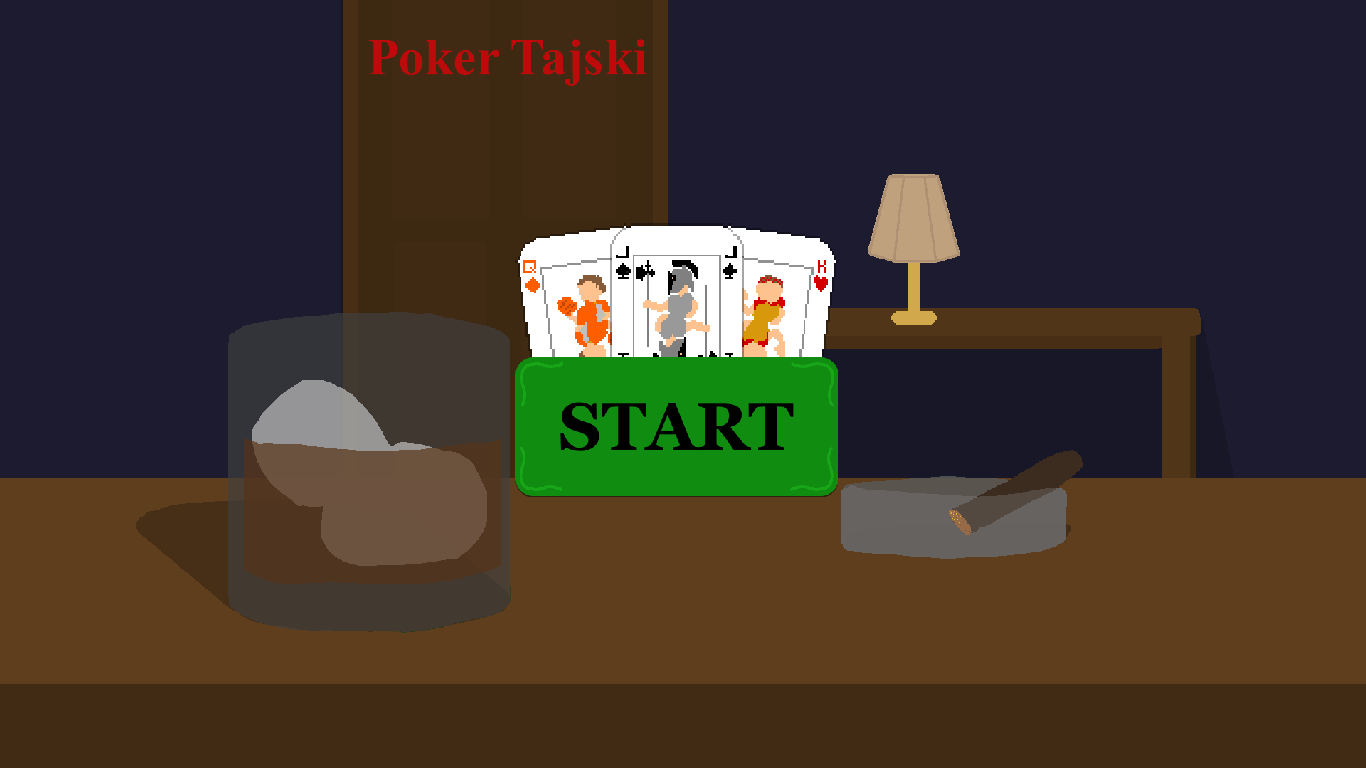
\includegraphics[width=0.5\textwidth]{start}
\caption{Ekran startowy}
\end{figure}

Ekran startowy zawiera jedynie jakże ujmującą grafikę oraz przycisk Start. Po jego naciśnięciu pojawia się ekran proszący o wpisanie nicku gracza. Po zatwierdzeniu go klawiszem Enter pojawią się opcje ``Stwórz'' i ``Dołącz''.

\begin{figure}[H]
\centering
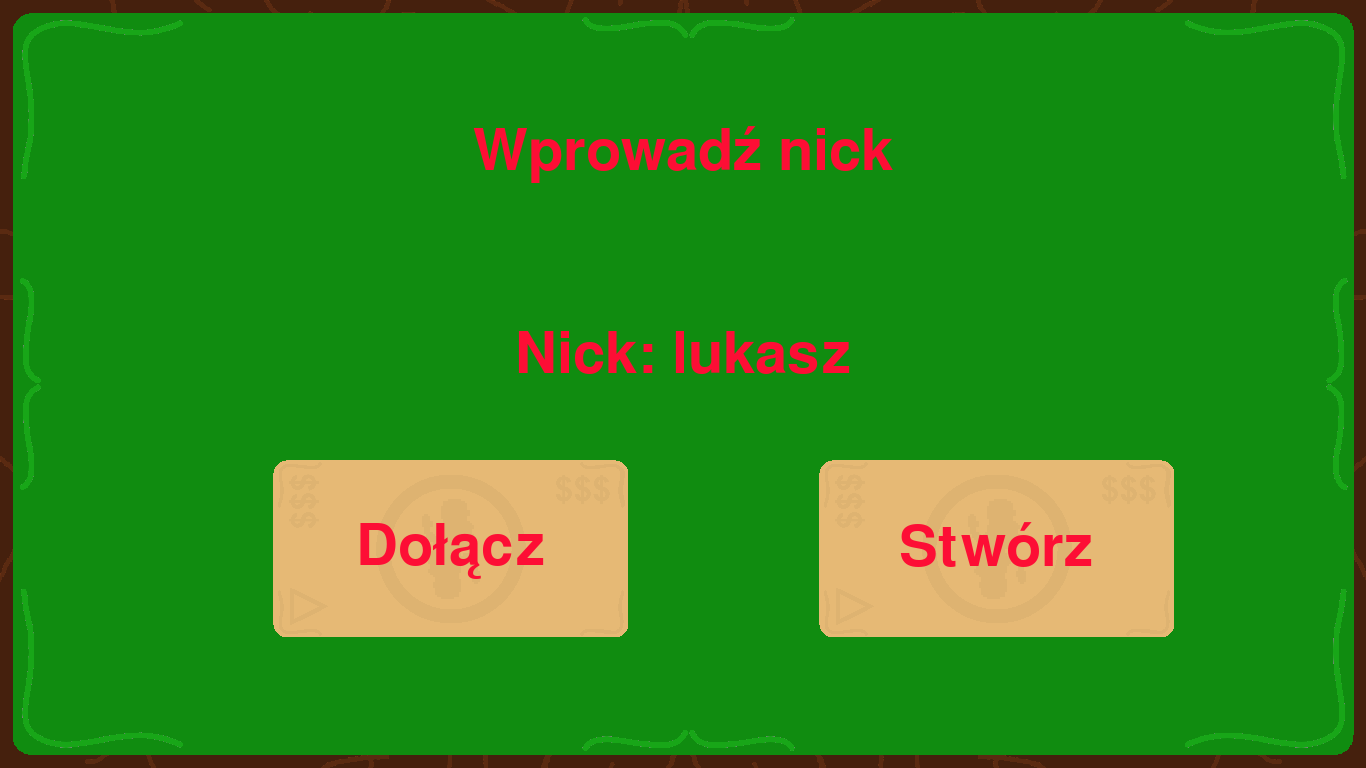
\includegraphics[width=0.5\textwidth]{wprowadzanie}
\caption{Widok po wprowadzeniu nicku}
\end{figure}

Po wybraniu opcji ``Stwórz'' pojawi się ekran z liczbą graczy obecnie znajdujących się przy stole oraz przycisk umożliwiający rozpoczęcie gry. Wyświetlana liczba oczywiście zmienia się zależnie od ilości graczy.

\begin{figure}[H]
\centering
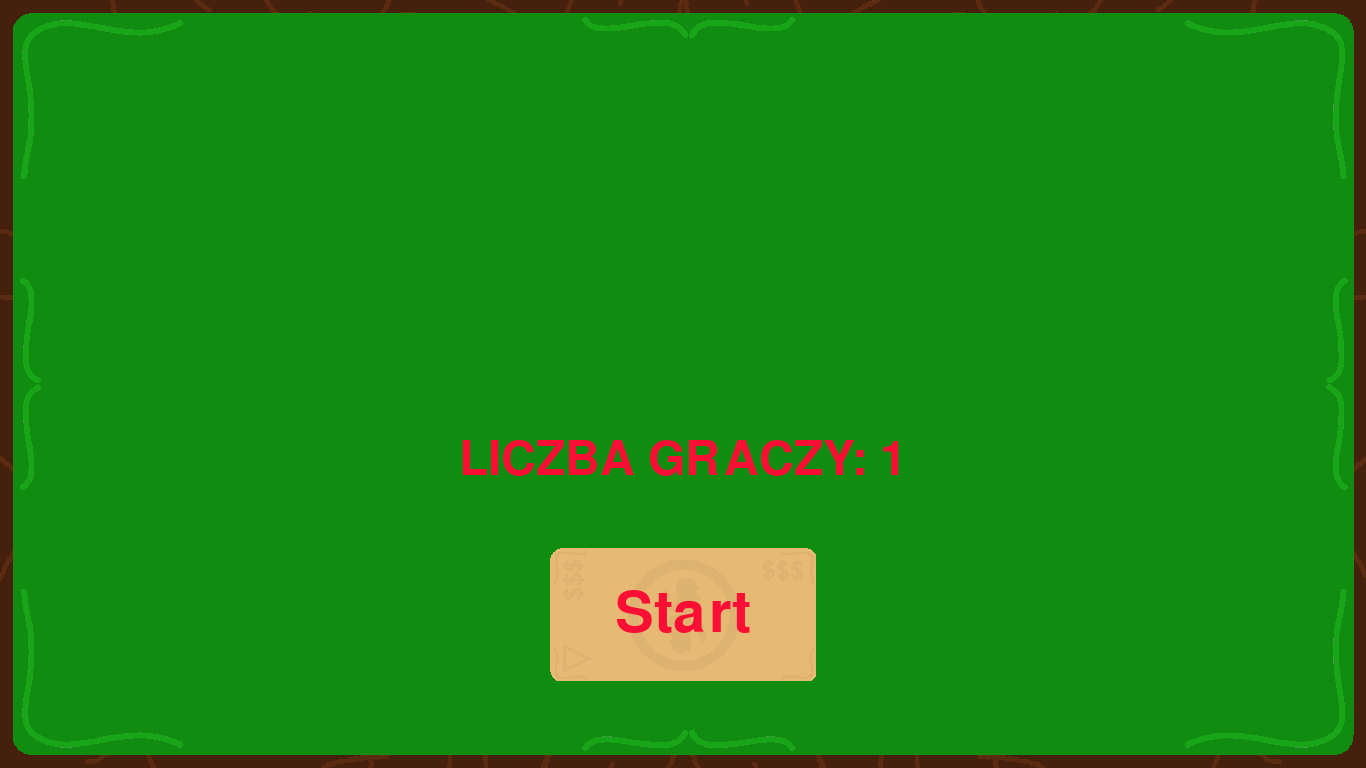
\includegraphics[width=0.5\textwidth]{oczekiwanie}
\caption{Ekran oczekiwania z opcją rozpoczęcia}
\end{figure}

Jeśli wybrano opcję ``Dołącz'', pojawi się lista dostępnych na danym serwerze stołów.

\begin{figure}[H]
\centering
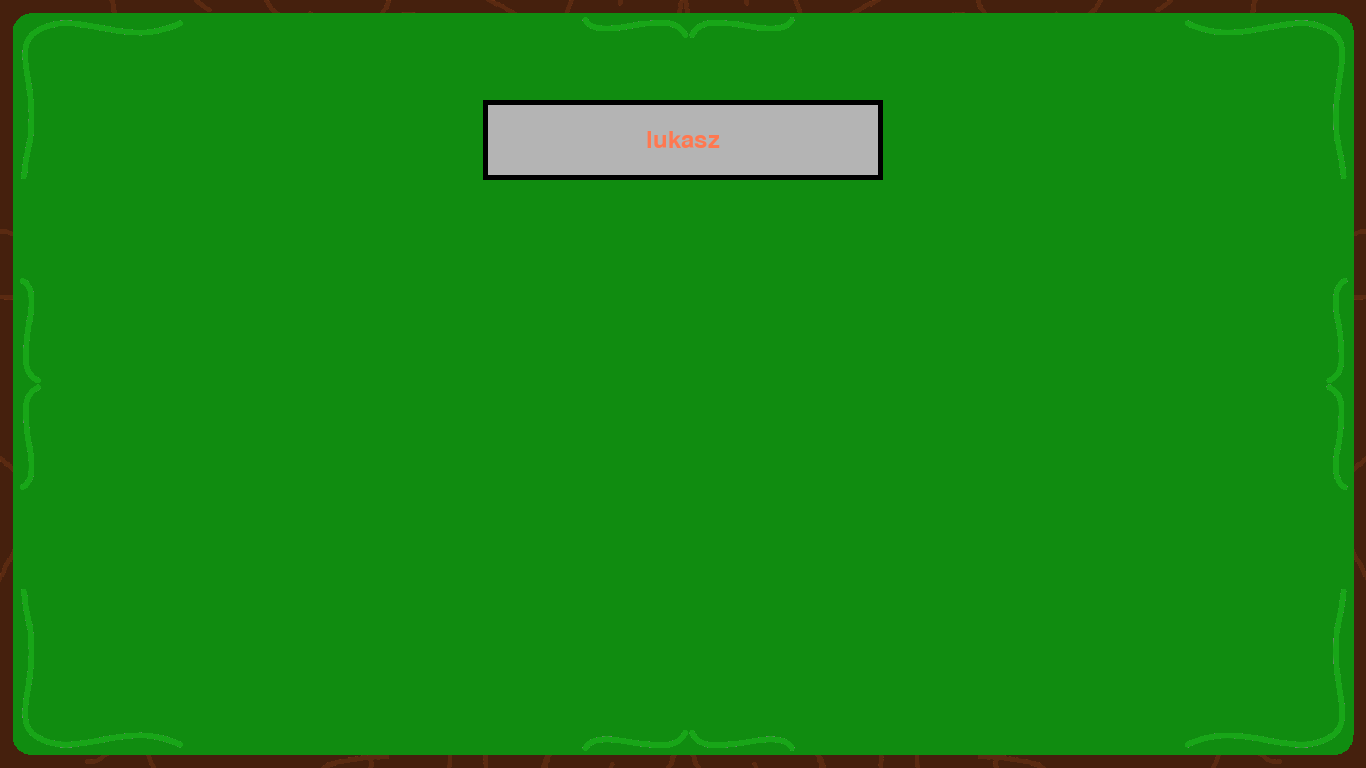
\includegraphics[width=0.5\textwidth]{dostepnestoly}
\caption{Lista dostępnych stołów}
\end{figure}

Wtedy po wybraniu stołu pojawia się ekran wyświetlający liczbę graczy przy stole i informujący o konieczności czekania.

\begin{figure}[h!]
\centering
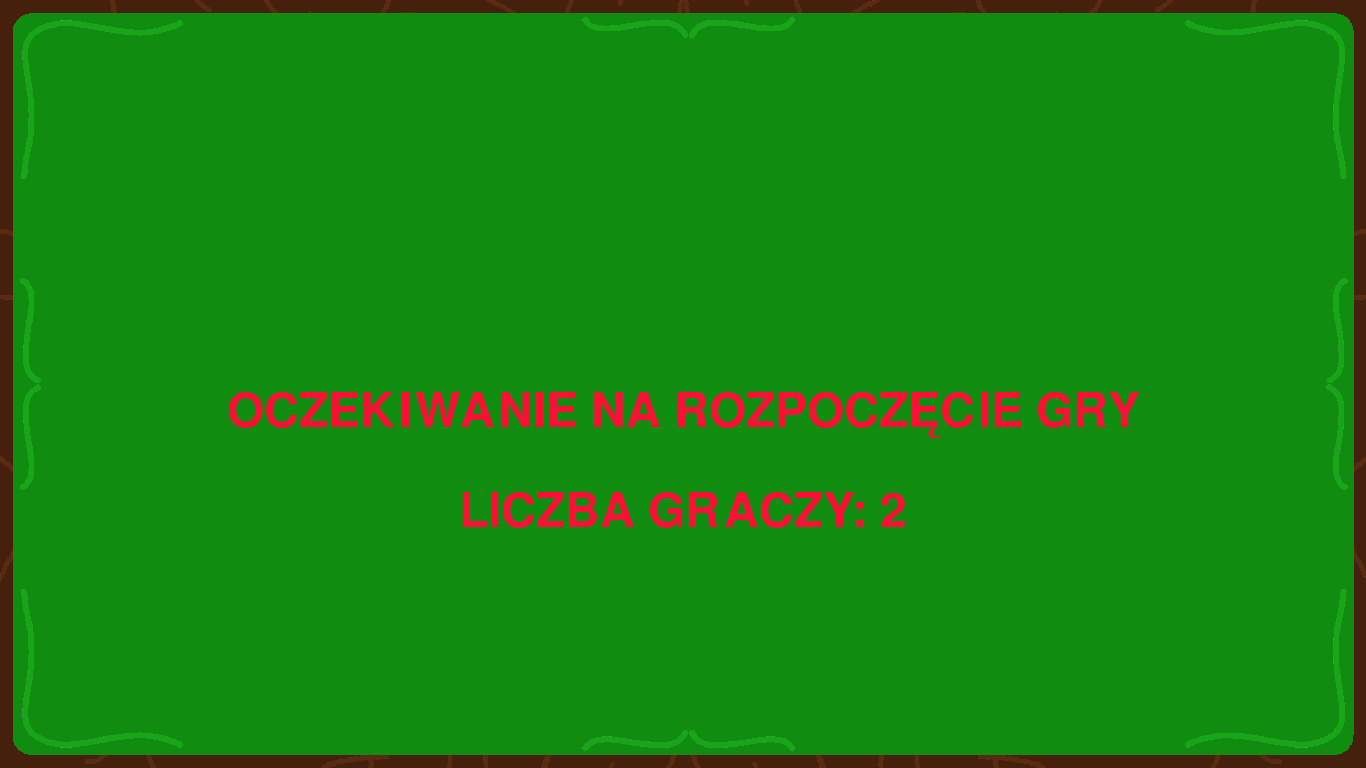
\includegraphics[width=0.7\textwidth]{stoloczekujacy}
\caption{Ekran oczekiwania bez opcji rozpoczęcia}
\end{figure}

Jeśli gracz, który stworzył stół, kliknie Start, wówczas włączy się animacja tasowania i rozdawania kart, po czym rozpocznie się gra. Interfejs wygląda blisko identycznie niezależnie od tego, czy jest to kolej danego gracza, czy nie - łatwo jednak rozpoznać, czyja jest to kolej, po obecności pomarańczowego przycisku CHECK w lewym dolnym rogu, który na ekranie danego gracza pojawia się tylko wtedy, kiedy jest jego kolej.
\newline

\begin{figure}[H]
\centering
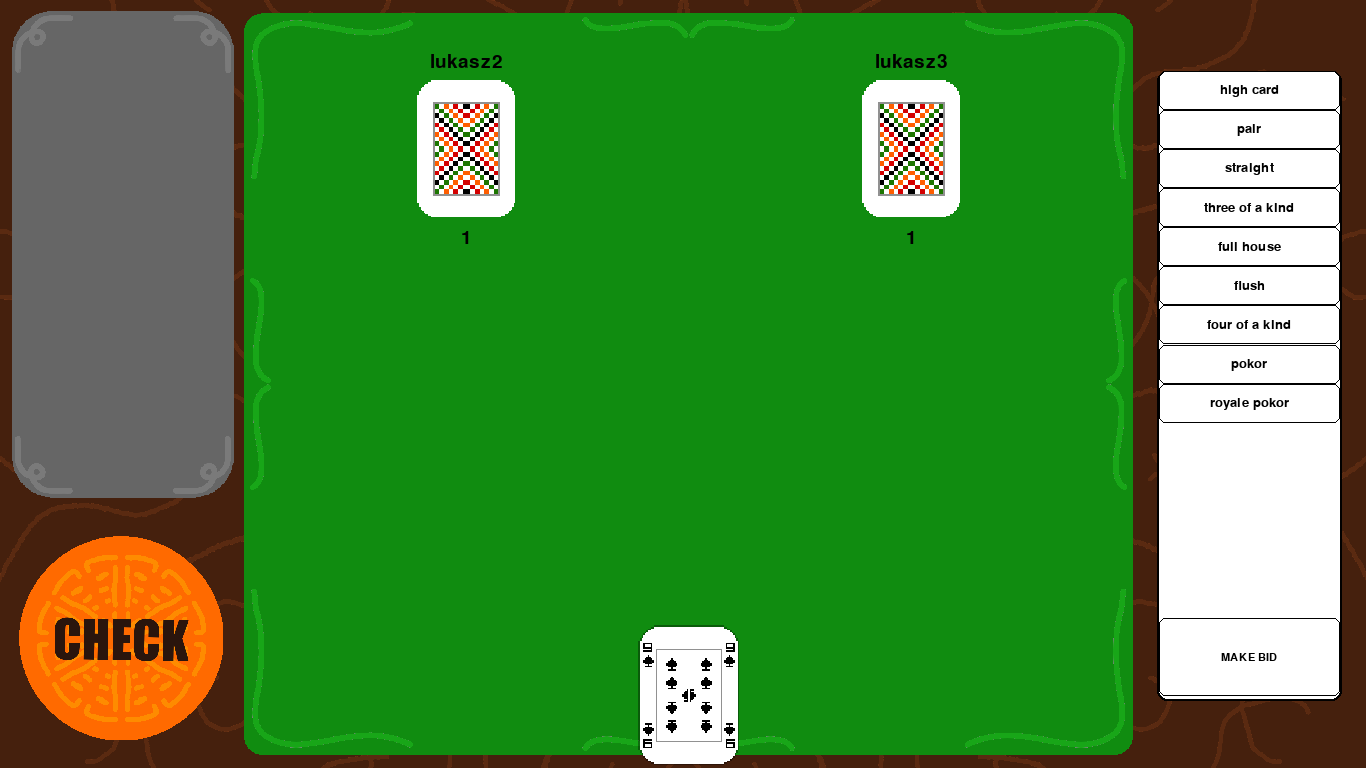
\includegraphics[width=\textwidth]{basicwidok}
\caption{Ekran gry - kolej danego gracza}
\end{figure}


W miarę gry, na szarym tle po lewej stronie będą pojawiać się złożone wcześniej odzywki. Umożliwia to śledzenie przebiegu gry.\\
Gra toczy się, dopóki któryś z graczy nie naciśnie przycisku CHECK, tym samym sprawdzając odzywkę poprzedniego gracza. Przycisk ten nie zareaguje na kliknięcie, jeśli żadna odzywka nie została podczas rundy złożona - w praktyce oznacza to, że gracz rozpoczynający rundę nie może od razu kliknąć CHECK.\\
Po pomyślnym (tzn. uznanym przez grę jako prawidłowe) sprawdzeniu, gracz, który przegrał, otrzyma komunikat ``Przegrałeś Synu!'', a reszta - ``Przegrał [\textit{nick}]'', gdzie \textit{nick} jest, rzecz jasna, nickiem gracza, który właśnie przegrał.

\begin{figure}[!htb]
   	\begin{minipage}{0.48\textwidth}
    	\centering
     	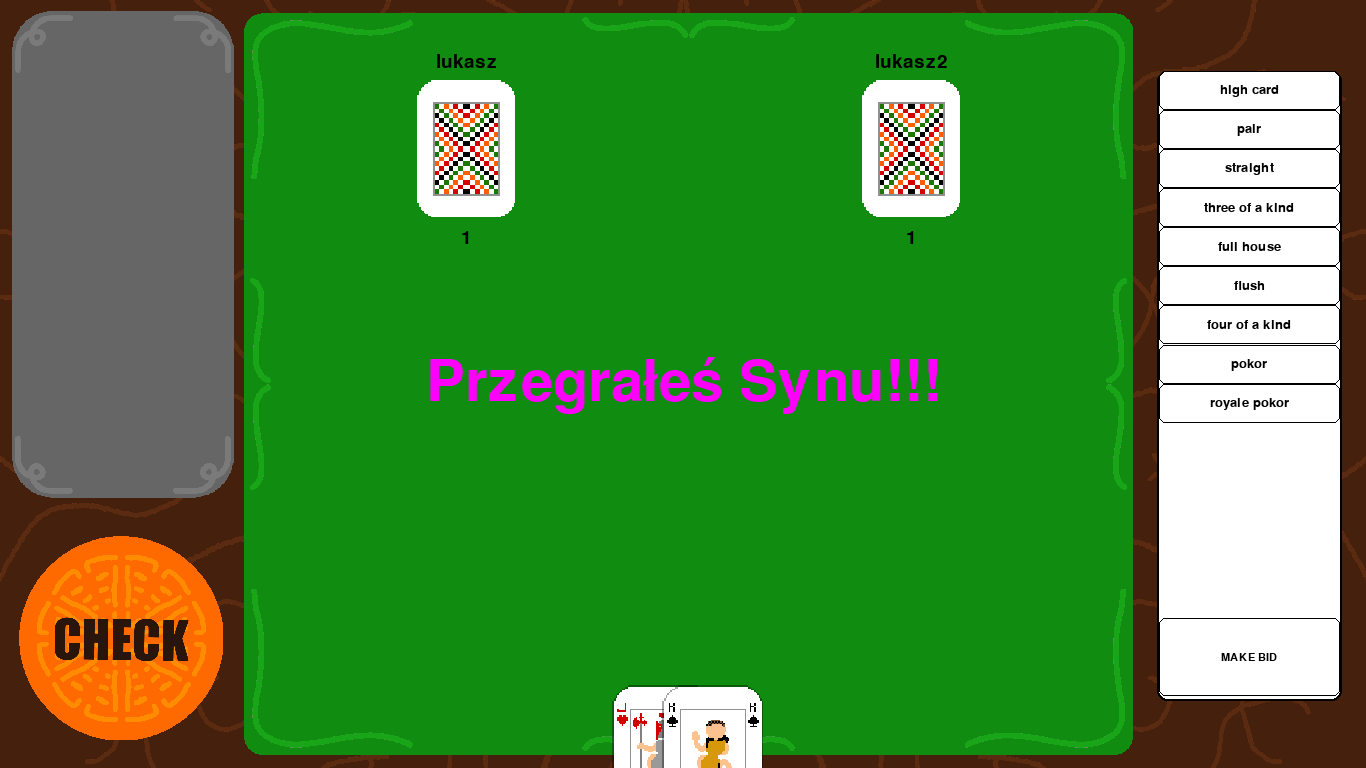
\includegraphics[width=\linewidth]{przegralessynu}
     	\caption{Widok przegranej danego gracza}
   	\end{minipage}\hfill
   	\begin{minipage}{0.48\textwidth}
     	\centering
     	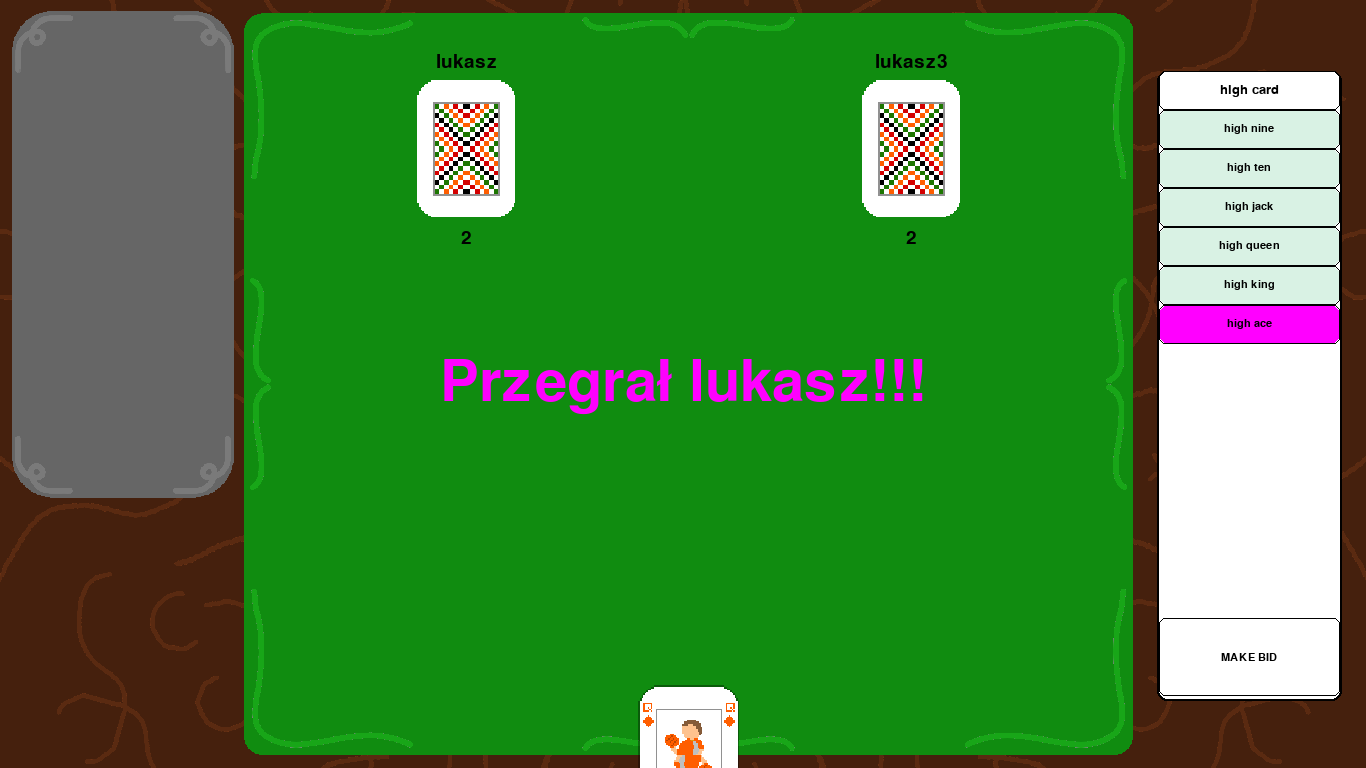
\includegraphics[width=\linewidth]{ktosprzegral}
     	\caption{Widok przegranej innego gracza}
   	\end{minipage}
\end{figure}

Komunikaty te będą się wyświetlały dopóki nie zostanie złożona odzywka w nowej rundzie. Również liczby kart (cyfry widoczne pod kartami przeciwników) zmienią się odpowiednio, tzn. liczba kart przegranego zwiększy się o 1.\\
Na Rys. 8 widać również, jak wygląda składanie odzywek - należy kliknąć w typ odzywki, który interesuje gracza, co odsłoni listę dostępnych. Następnie należy kliknąć konkretną odzywkę, która podświetli się na różowo, oraz kliknąć ``MAKE BID''. Odzywki niedostępne, choć będzie można zobaczyć ich listę, będą wyświetlały się na szaro i nie będą reagować na klikanie. Jeśli gracz się rozmyślił i chce zmienić typ składanej odzywki, musi jeszcze raz kliknąć listę, aby ją najpierw zwinąć.

W momencie \textit{przegranej} któregokolwiek z graczy, czyli jeśli ktokolwiek przekroczy dopuszczalną liczbę posiadanych kart, gracz ten zostaje usuwany z gry - nie są mu już rozdawane karty, choć może nadal przebywać przy stole i obserwować dalszy przebieg rozgrywki. Dla innych graczy jest on nadal widoczny, lecz liczba jego kart widnieje jako 0.

\begin{figure}[H]
\centering
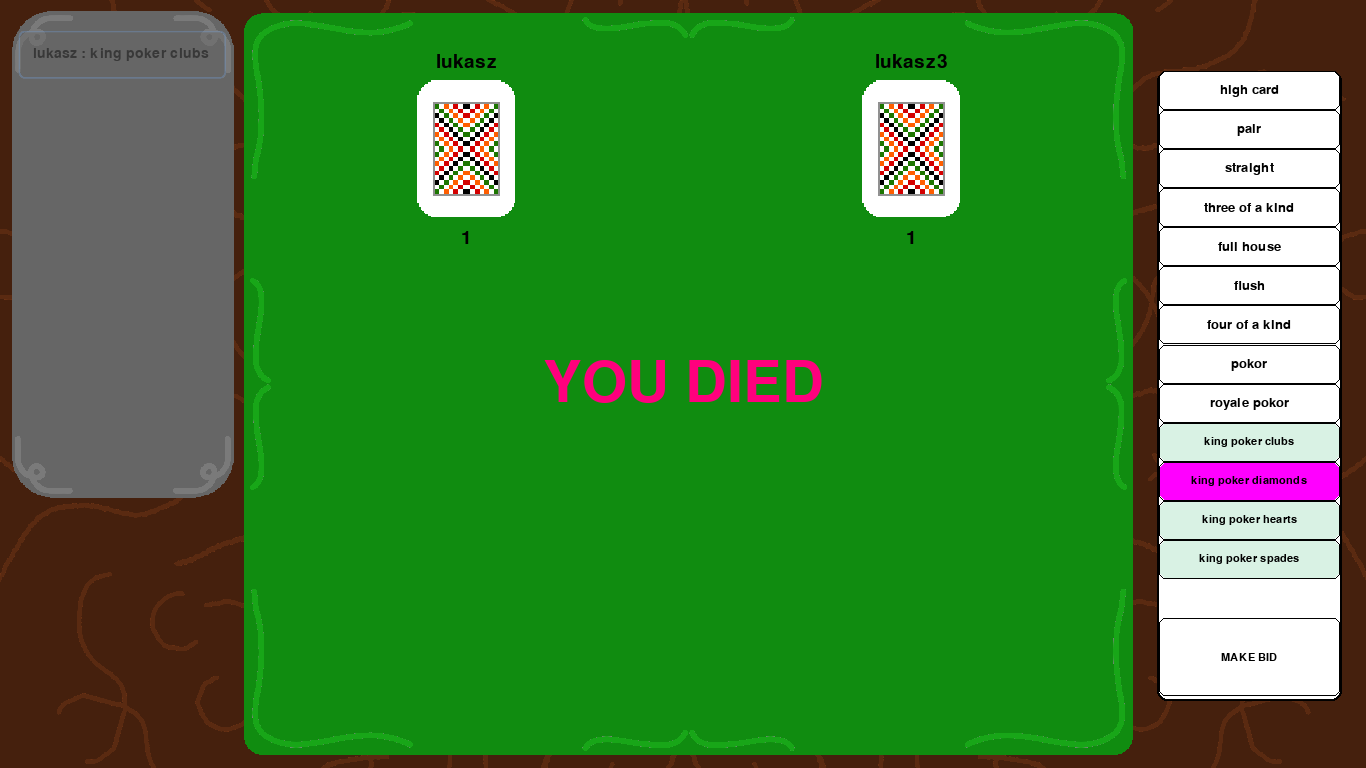
\includegraphics[width=0.4\textwidth]{youdied}
\caption{Widok gracza który odpadł z gry}
\end{figure}

\end{document}